\documentclass[10pt]{report}
\usepackage[a4paper,bindingoffset=0.2in,
			left=0.5in,right=0.5in,top=1in,bottom=1in,
			footskip=.25in]{geometry}
\usepackage[affil-it]{authblk}
\usepackage[utf8]{inputenc}
\usepackage{listings}
\usepackage{color}
\usepackage{xcolor}
\usepackage{pdfpages}
\usepackage{graphicx}
\graphicspath{{./graphics/}}
\usepackage{textcomp}
\usepackage{hyperref}
\usepackage{dirtree}
\usepackage{minted}
\usepackage{footnotebackref}
\usepackage{amsmath}
\usepackage{ragged2e}

\definecolor{codegreen}{rgb}{0,0.6,0}
\definecolor{codegray}{rgb}{0.5,0.5,0.5}
\definecolor{codepurple}{rgb}{0.58,0,0.82}
\definecolor{backcolour}{rgb}{1.0,1.0,1.0}

%% Title Definition Packages & Commands %%
\usepackage{titlesec}
\titleformat
{\chapter}
[display]
{\bfseries\LARGE}
{Chapter \thechapter}
{0pt}
{
	\rule{\textwidth}{1pt}
	\centering
}
[
\rule{\textwidth}{0.3pt}
]
\titlespacing{\chapter}{0pt}{10pt}{10pt}

\renewcommand{\paragraph}[1]{\paragraph{#1}\mbox{}\\}
%%%%
%% Box Packages & Commands %%
\usepackage{lmodern}
\usepackage[most]{tcolorbox}
\usepackage{tabularx}
\usepackage{colortbl} 
\newcolumntype{Y}{>{\centering\arraybackslash}X}
\newtcolorbox[blend into=tables]{colortable}[2][]{
	colback=white,
	tabularx*={\renewcommand{\arraystretch}{1.0}}{Y|Y|Y|Y|Y|Y},title={#2},boxrule=0.8pt, center title
}
\newtcolorbox[blend into=figures]{blockfigure}[2][]
{
	colback=white,
	float=!htbp,
	boxsep=1pt,
	left=1pt,
	right=1pt,
	top=1pt,
	bottom=1pt,
	center title,
	%%lifted shadow={1mm}{-2mm}{3mm}{0.1mm}{black!50!white},
	title={#2},
	every float=\centering,
	#1
}
\newtcolorbox[blend into=figures]{inlinefigure}[2][]
{
	colback=white,
	boxsep=0.5pt,
	left=1pt,right=1pt,
	top=1pt,
	bottom=1pt,
	center title,
	%%lifted shadow={1mm}{-2mm}{3mm}{0.1mm}{black!50!white},
	title={#2},
	every float=\centering,
	#1
}
%%%%

\newcommand{\folder}[2]{}

\newcommand\tab[1][1cm]{\hspace*{#1}}


\makeatletter
\newcommand\footnoteref[1]{\protected@xdef\@thefnmark{\ref{#1}}\@footnotemark}
\makeatother

\lstdefinestyle{mystyle}{
	backgroundcolor=\color{backcolour},   
	commentstyle=\color{codegreen},
	keywordstyle=\color{magenta},
	numberstyle=\tiny\color{codegray},
	stringstyle=\color{codepurple},
	basicstyle=\scriptsize,
	breakatwhitespace=false,         
	breaklines=true,                 
	captionpos=b,                    
	keepspaces=true
}


\lstset{style=mystyle}
\begin{document}
	\begin{titlepage}
		\begin{center}
			
\includegraphics[width=0.6\textwidth]{UnivAQ-logo}\\[1cm]
			{\LARGE University of L'Aquila}\\[0.5cm]
			{\large Department of Information Engineering, Computer Science and Mathematics}\\[0.5cm]
			\rule{\linewidth}{0.5mm} \\[0.4cm]
			{\huge \bfseries NavibusMercatoriis:\\ A Database for a Mercantile Shipping Company \\[0.4cm] }
			\rule{\linewidth}{0.5mm} \\[0.1cm]
			\noindent
			{\large  \textsc{Databases - Lab Module - Final Project}
				\vspace{-0.04cm} \\[0.01cm] }
			\rule{\linewidth}{0.5mm} \\[0.1cm]
			\noindent
			\begin{tcbraster}[raster columns=2,raster rows=1,
				enhanced,size=small,fit algorithm=hybrid* ]
				\begin{tcolorbox}[
					colback=white,
					sharp corners = northwest,
					title={Student}
					]
					\large
					\emph{Name :} \\[0.2cm]
					\tab Aly \textsc{Shmahell}\\[0.2cm]
				\end{tcolorbox}
				\begin{tcolorbox}[
					colback=white,
					sharp corners = northwest,
					title = {Supervisor}
					]
					\large
					\emph{Name :} \\[0.2cm]
					\tab Prof.~Pierluigi \textsc{Pierini}\\[0.2cm]
				\end{tcolorbox}
			\end{tcbraster}
			\vfill
			Jan 9th 2018
		\end{center}
	\end{titlepage}
\chapter*{Abstract}
\begin{center}
	\begin{minipage}{0.8\textwidth}
		\justify
		As part of a lab course on databases, I, the student, was tasked with designing a database for a mercantile shipping company, starting from specifications given by the supervisor, according to industry standards. In this document I showcase the four stages of design, along with the design decisions that are made beforehand. Great care is given into finding optimal solutions, but in some extreme cases a local optima is chosen for conformity purposes (the solution conforms best to the design stage), for practicality or for highlighting the optimal solution.
	\end{minipage}
	\vfill
	\begin{minipage}{0.8\textwidth}
		\begin{center}
			\url{https://github.com/AlyShmahell/NavibusMercatoriis}
		\end{center}
	\end{minipage}
\end{center}
		
\newpage
\chapter*{Design Decisions}

\begin{colortable}{Design Tool}
	\textbf{Question} & Which design tool to choose? \\\hline
	\textbf{Options} & \begin{itemize} 
							\item Dia  
							\item MySQL Workbench
						\end{itemize} \\\hline
	\textbf{Criteria} & \begin{itemize} 
							\item being up to date  
							\item offering ER models
						\end{itemize} \\\hline
	\textbf{Evaluation}  & \begin{itemize}
								\item MySQL Workbench satisfies both criteria, it also comes equipped with SQL scripting, python scripting, SQL database connection, and an SQL linter/debugger.
								\item Dia is outdated and lacks features.
							\end{itemize}  \\\hline
	\textbf{Choice} &  MySQL Workbench
\end{colortable}

\begin{colortable}{Testing Tool}
	\textbf{Question} & Which testing tool to choose? \\\hline
	\textbf{Options} & \begin{itemize} 
		\item phpmyadmin  
		\item adminer
	\end{itemize} \\\hline
	\textbf{Criteria} & \begin{itemize} 
		\item being up to date.
		\item offering PL/SQL support.
	\end{itemize} \\\hline
	\textbf{Evaluation}  & \begin{itemize}
		\item adminer satisfies both criteria.
		\item phpmyadmin lacks proper support for delimiters in stored procedures.
	\end{itemize}  \\\hline
	\textbf{Choice} &  adminer
\end{colortable}


\newpage
\chapter*{Stage 1: Conceptual Design}
\begin{normalsize}
	For the Conceptual Schema I used Crow's Foot notation, mainly because it is the one adopted by the CASE tool I chose (MySQL WorkBench).\\
	
	With this notation, relationships cannot have attributes. When necessary, relationships are promoted to entities. However, when relationships are not promoted to entities, they represent external identifiers as foreign key or index attributes which become present in both entities on the left and right hand side.\\
	
	This results in the following:
	\begin{itemize}
		\item adaptation of external identifiers into foreign keys early on in the conceptual design stage.
		\item selection of primary identifiers can also be done in the conceptual design stage.
		\item many-to-many relationships are replaced with entities in the conceptual design stage.
	\end{itemize}
\end{normalsize}

\begin{blockfigure}{Conceptual ERD with Crow's Foot (IE) Notation}
	\begin{center}
		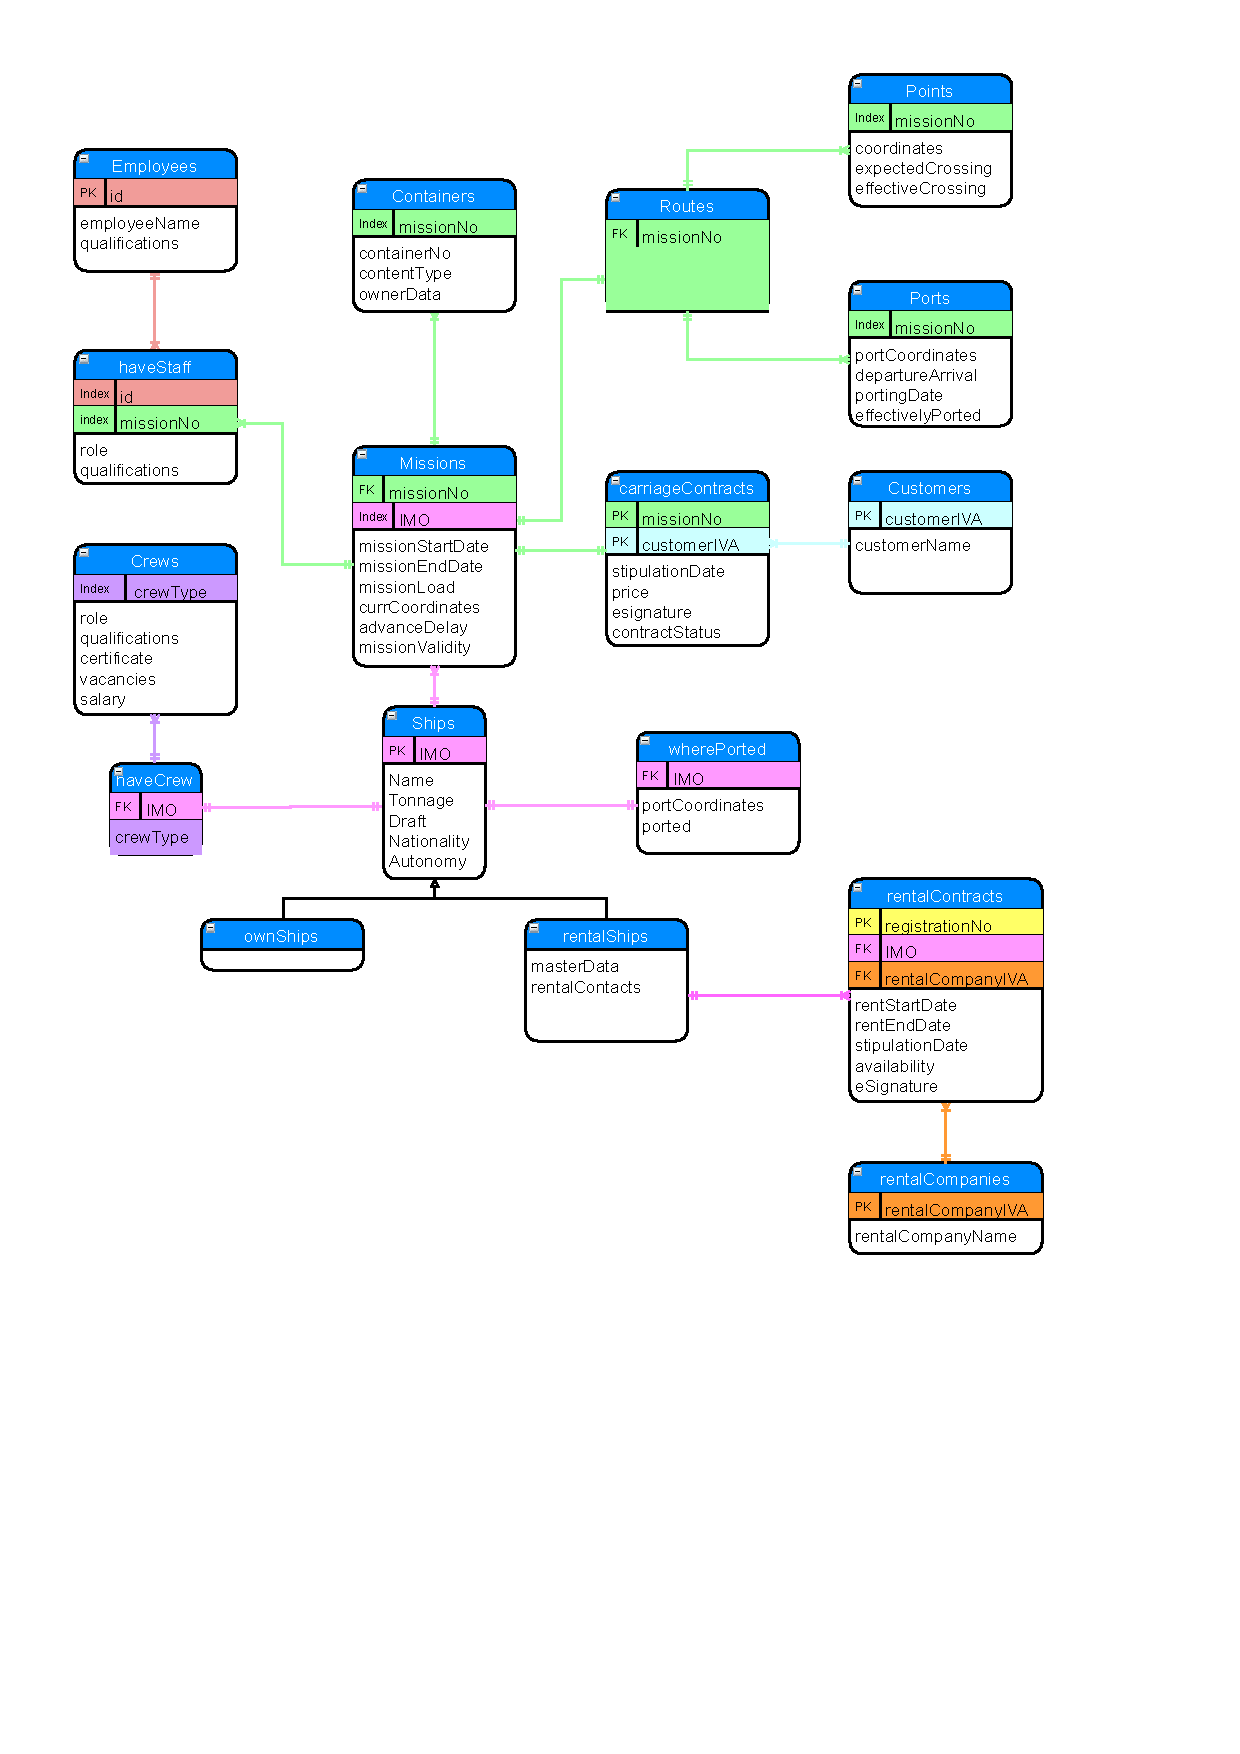
\includegraphics[trim=0cm 8cm 0cm 1cm,clip=true, width=.6\textwidth]{mercantileShips-Conceptual.pdf}
	\end{center}
\end{blockfigure}

\chapter*{Stage 2: Logical Design}
\begin{center}
	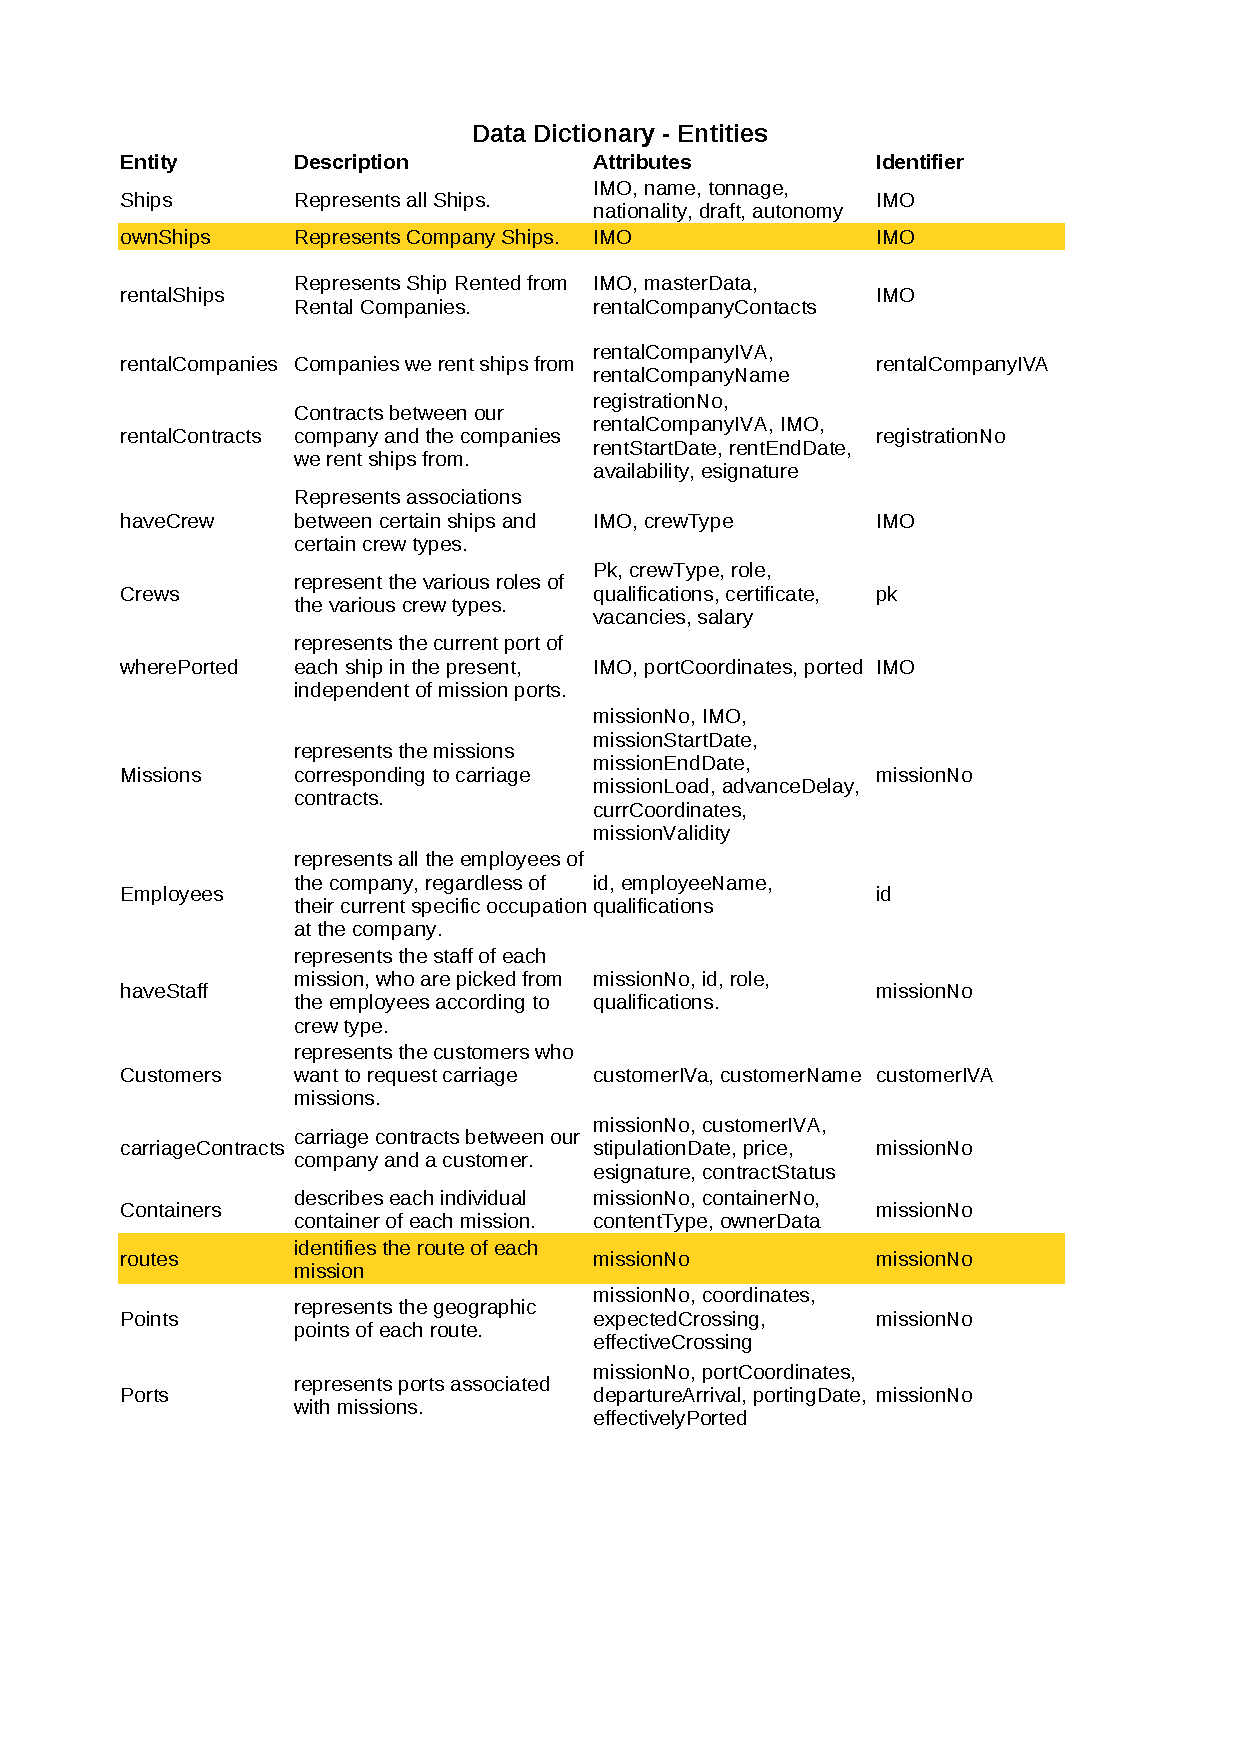
\includegraphics[trim=0cm 4cm 0cm 0cm,clip=true,height=.85\textheight, width=\textwidth]{DataDictionary1.pdf}
\end{center}
\newpage
\begin{center}
	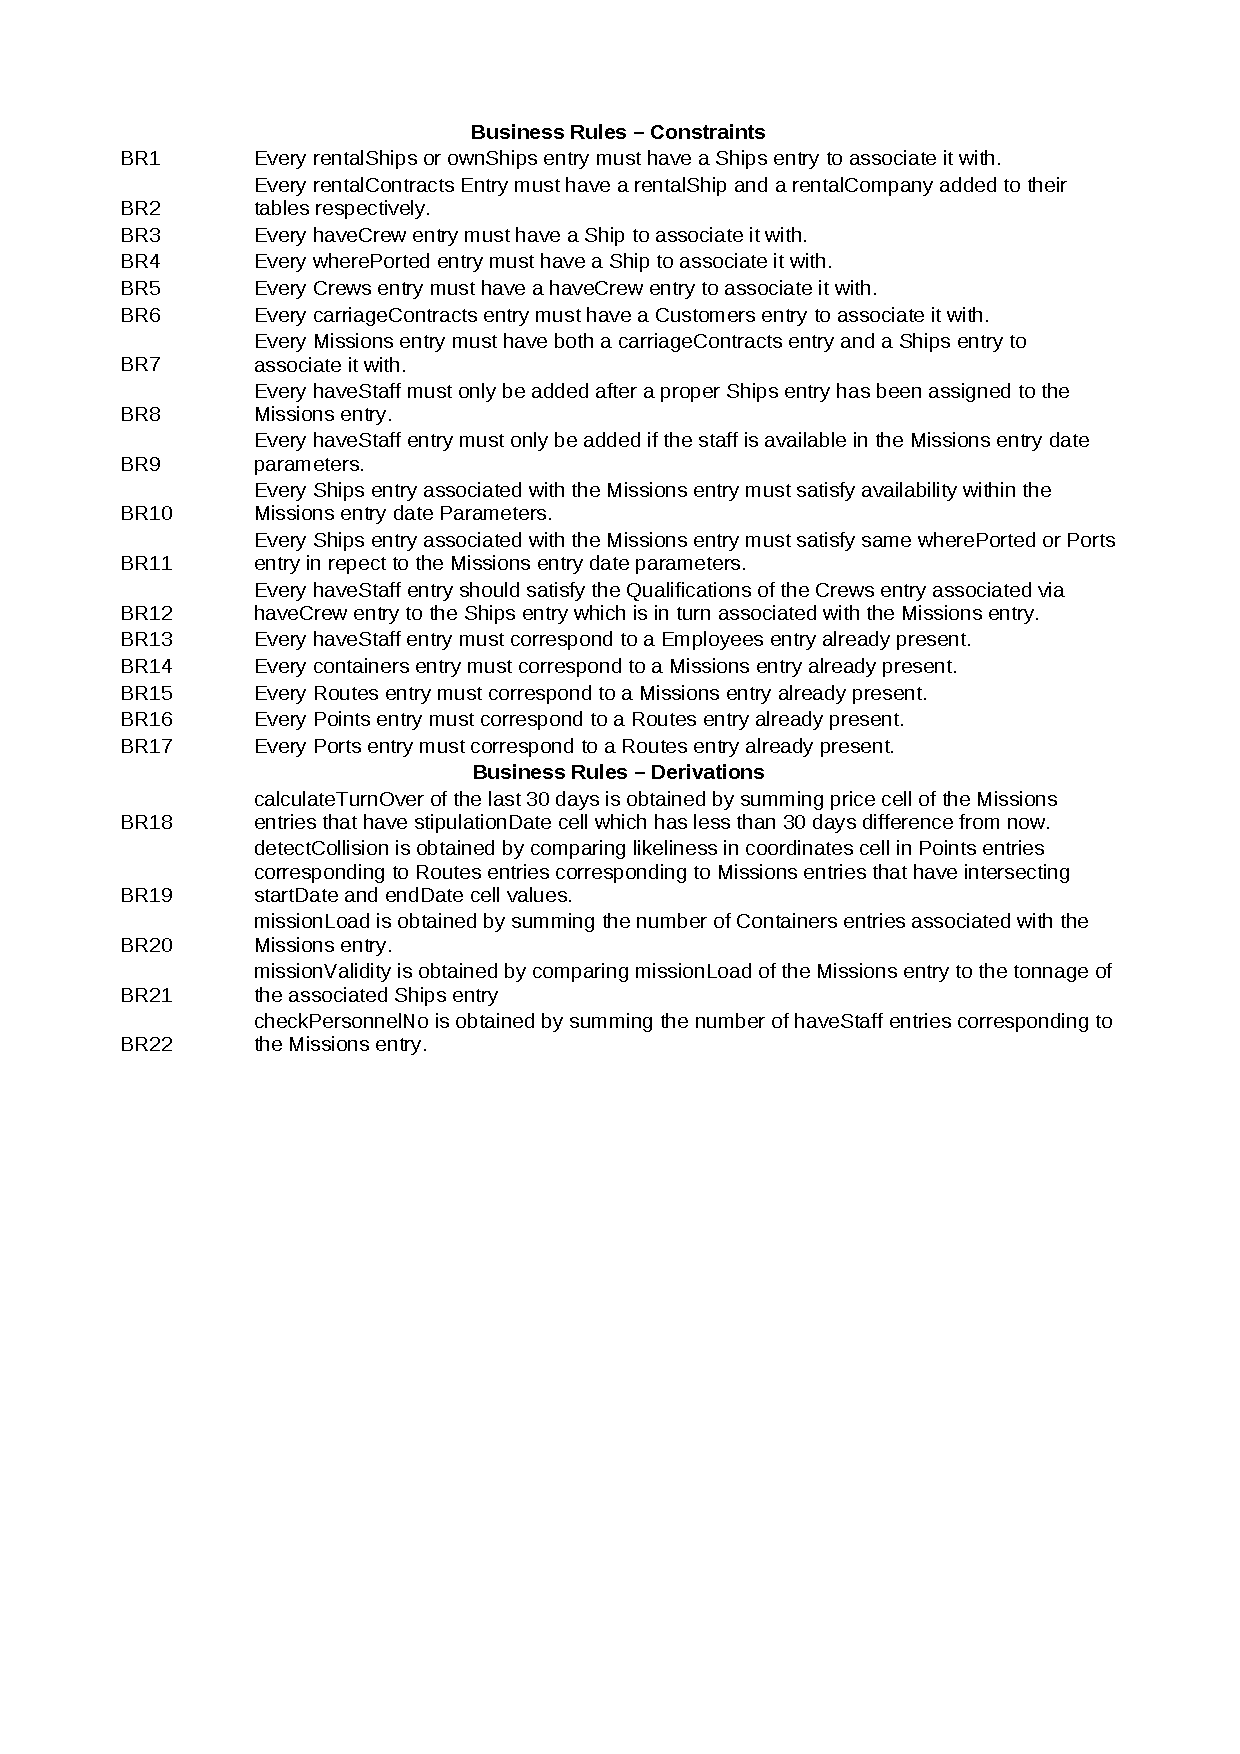
\includegraphics[trim=2cm 10cm 0cm 0cm,clip=true, height=.85\textheight, width=\textwidth]{BusinessRules.pdf}
\end{center}
\newpage
\begin{center}
	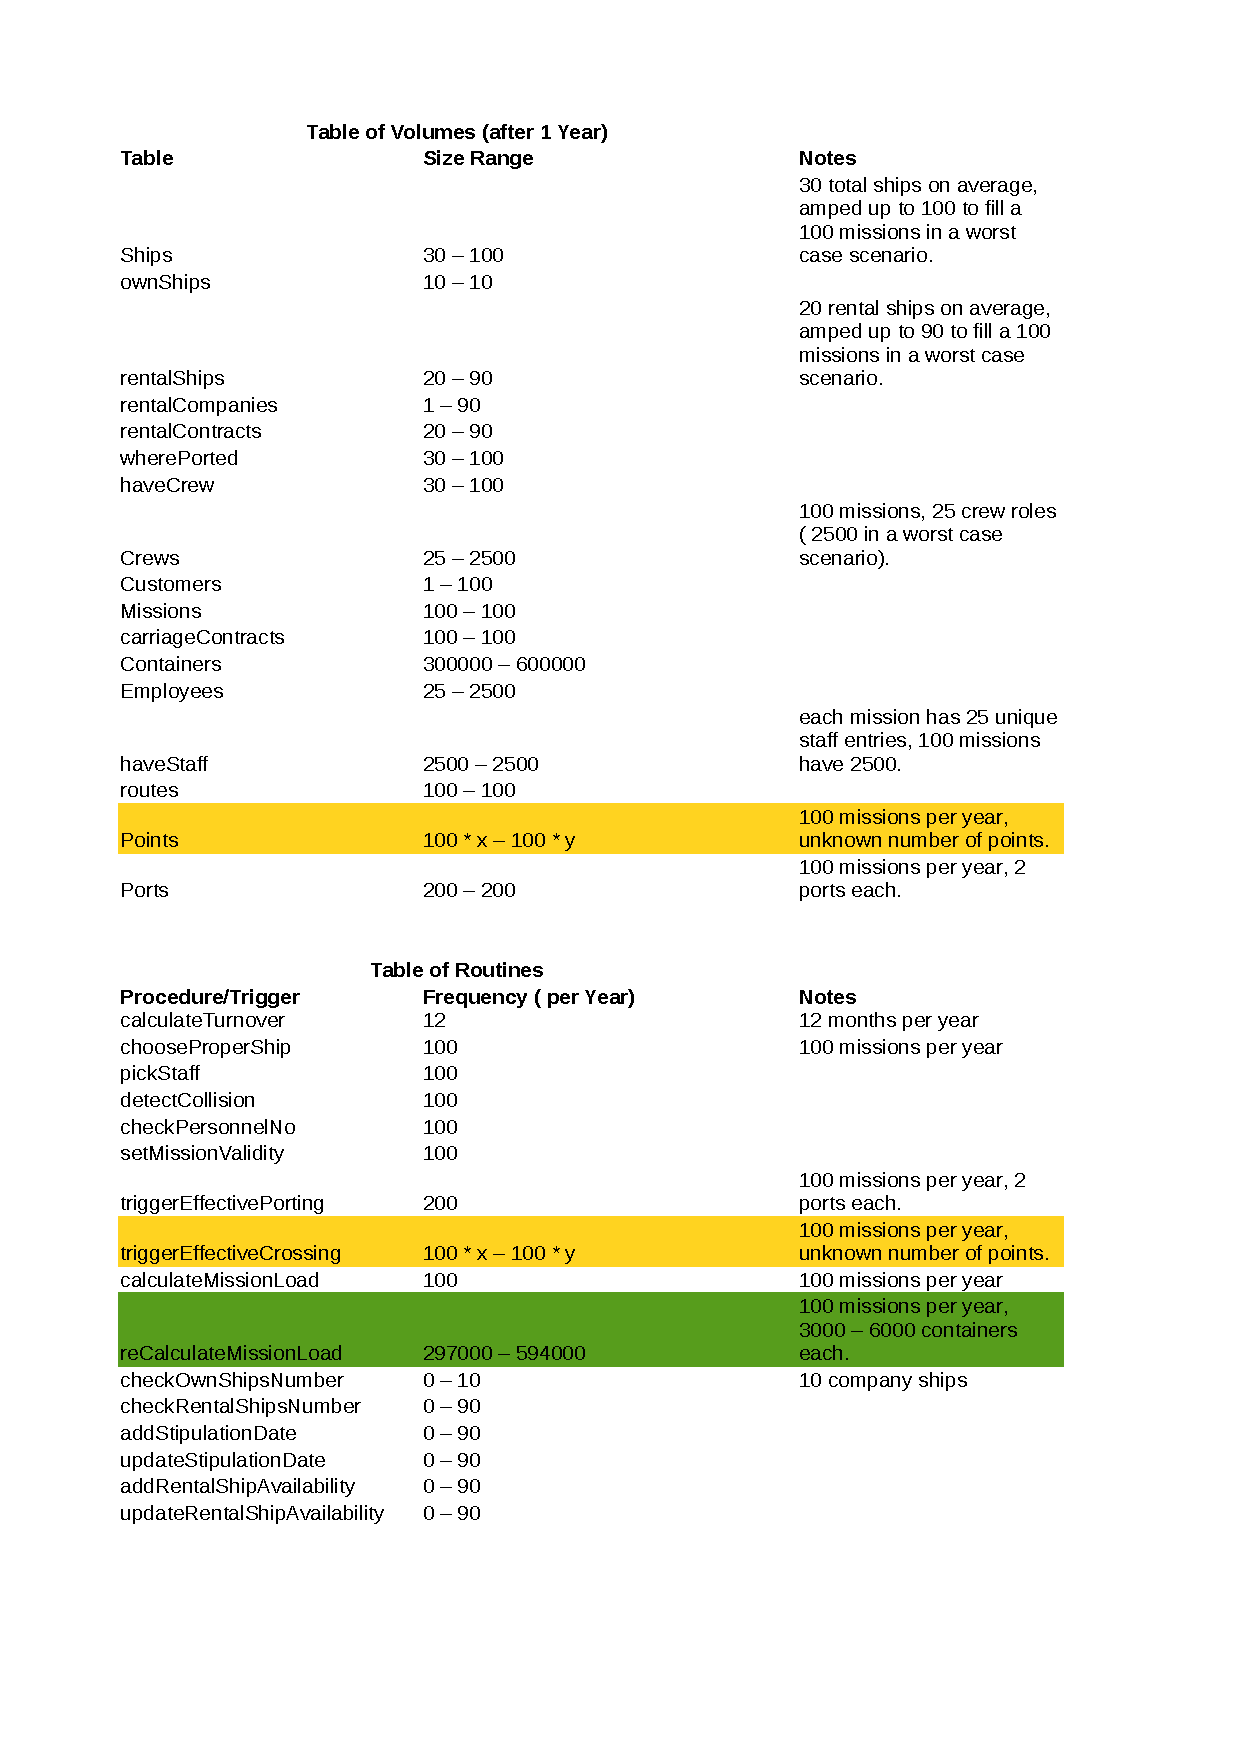
\includegraphics[trim=1cm 3cm 2cm 0cm,clip=true, height=.85\textheight, width=\textwidth]{Volumes.pdf}
\end{center}
\newpage
\begin{center}
	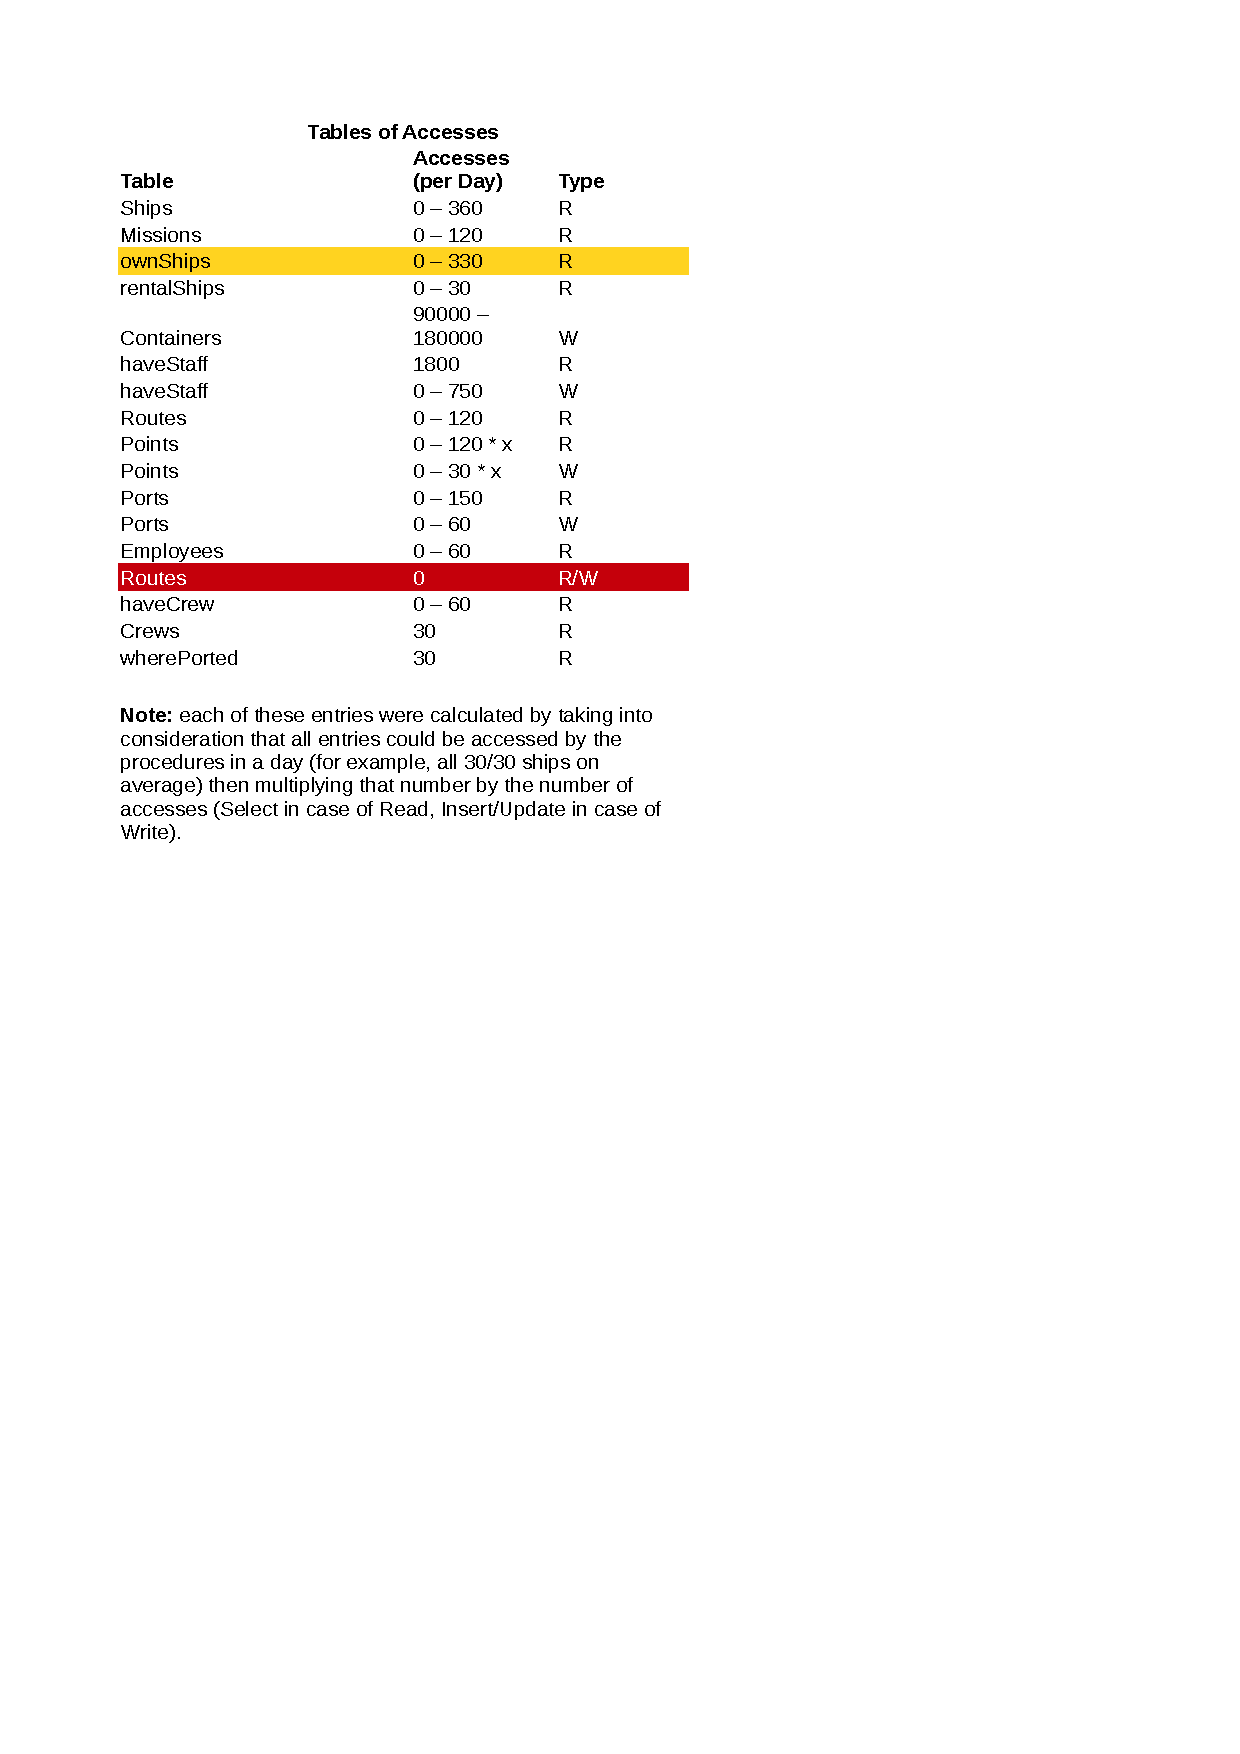
\includegraphics[trim=2cm 12cm 9cm 0cm,clip=true, height=.85\textheight, width=\textwidth]{Accesses.pdf}
\end{center}
\newpage
\chapter*{Stage 3: Normalization}
Removal of a generalizations was done following the \textbf{"Substitution of the generalization with relationships"} method.\\

The resulting translated tables were as the following:
\begin{flushleft}
	Ships(\underline{IMO}, name, tonnage, draft, autonomy, nationality)\\
	ownShips(\underline{IMO})\\
	rentalShips(\underline{IMO}, masterData, rentalContacts)\\
	rentalCompanies(\underline{rentalCompanyIVA},rentalCompanyName)\\
	rentalContracts(\underline{registrationNo}, rentalCompanyIVA, IMO, rentStartDate, rentEndDate, availability, eSignature)\\
	wherePorted(\underline{IMO}, portCoordinates, ported)\\
	haveCrew(\underline{IMO}, crewType)\\
	Crews(\textit{crewType}, role, qualifications, certificate, vacancies, salary)\footnote{\label{italic1}attributes in italic represent indexes}\\
	Missions(\underline{missionNo}, IMO, missionStartDate, missionEndDate, missionLoad, currCoordinates, advanceDelay, missionValidity)\\
	Customers(\underline{customerIVA}, customerName)\\
	Employees(\underline{id}, employeeName, qualifications)\\
	carriageContracts(\underline{missionNo}, customerIVA, stipulationDate, price, eSignature, contractStatus)\\
	haveStaff (\textit{id}, \textit{missionNo}, role, qualifications)\footnoteref{italic1}\\
	Containers(\textit{missionNo}, containerNo, contentType, ownerData)\footnoteref{italic1}\\
	Routes(\underline{missionNo})\\
	Ports(\textit{missionNo}, portCoordinates, departureArrival, portingDate, effectivelyPorted)\footnoteref{italic1}\\
	Points(\textit{missionNo}, coordinates, expectedCrossing, effectiveCrossing)\footnoteref{italic1}\\
\end{flushleft}
The resulting translated foreign key relations are as the following:
\begin{flushleft}
	\verb|fk_rentalContracts_rentalCompanies1|(rentalContracts.rentalCompanyIVA, rentalCompanies.rentalCompanyIVA)\\
	\verb|fk_rentalContracts_rentalShips1|(rentalContracts.IMO, rentalShips.IMO)\\
	\verb|fk_rentalShips_Ships1|(rentalShips.IMO,Ships.IMO)\\
	\verb|fk_ownShips_Ships1|(ownShips.IMO, Ships.IMO)\\
	\verb|fk_wherePorted_Ships1|(wherePorted.IMO, Ships.IMO)\\
	\verb|fk_haveCrew_Ships1|(haveCrew.IMO, Ships.IMO)\\
	\verb|fk_Crews_haveCrew1|(Crews.crewType, haveCrews.crewType)\\
	\verb|fk_Missions_Ships1|(Missions.IMO, Ships.IMO)\\
	\verb|fk_carriageContract_Customer1|(carriageContracts.customerIVA, Customers.customerIVA)\\
	\verb|fk_Missions_carriageContracts1|(Missions.MissionNo, carriageContracts.MissionNo)\\
	\verb|fk_haveStaff_Employees1|(haveStaff.id, Employees.id)\\
	\verb|fk_haveStaff_Missions1|(haveStaff.missionNo, Missions.missionNo)\\
	\verb|fk_Loads_Missions1|(Containers.missionNo, Missions.missionNo)\\
	\verb|fk_Routes_Missions1|(Routes.missionNo, Missions.missionNo)\\
	\verb|fk_Ports_Routes1|(Ports.missionNo, Routes.missionNo)\\
	\verb|fk_Points_Routes1|(Points.missionNo, Routes.missionNo)\\
\end{flushleft}
\textbf{Notes on Efficiency}\\
As we can see in the table of accesses, the \textbf{Routes} table is accessed very rarely, and it imposes an un-necessary structural redundancy (only contains missionNo), therefor should be deleted and substituted with the \textbf{"missionNo"} attribute in the \textbf{Missions} table.\\
Also, the \textbf{ownShips} table is accessed as frequently as the \textbf{Ships} table, but poses another un-necessary structural redundancy, therefor should be deleted and substituted with a binary attribute \textbf{"isOwn"} in the \textbf{Ships} table.
\newpage

\begin{inlinefigure}{Relational EERD with Crow's Foot (IE) Notation}
	\begin{center}
		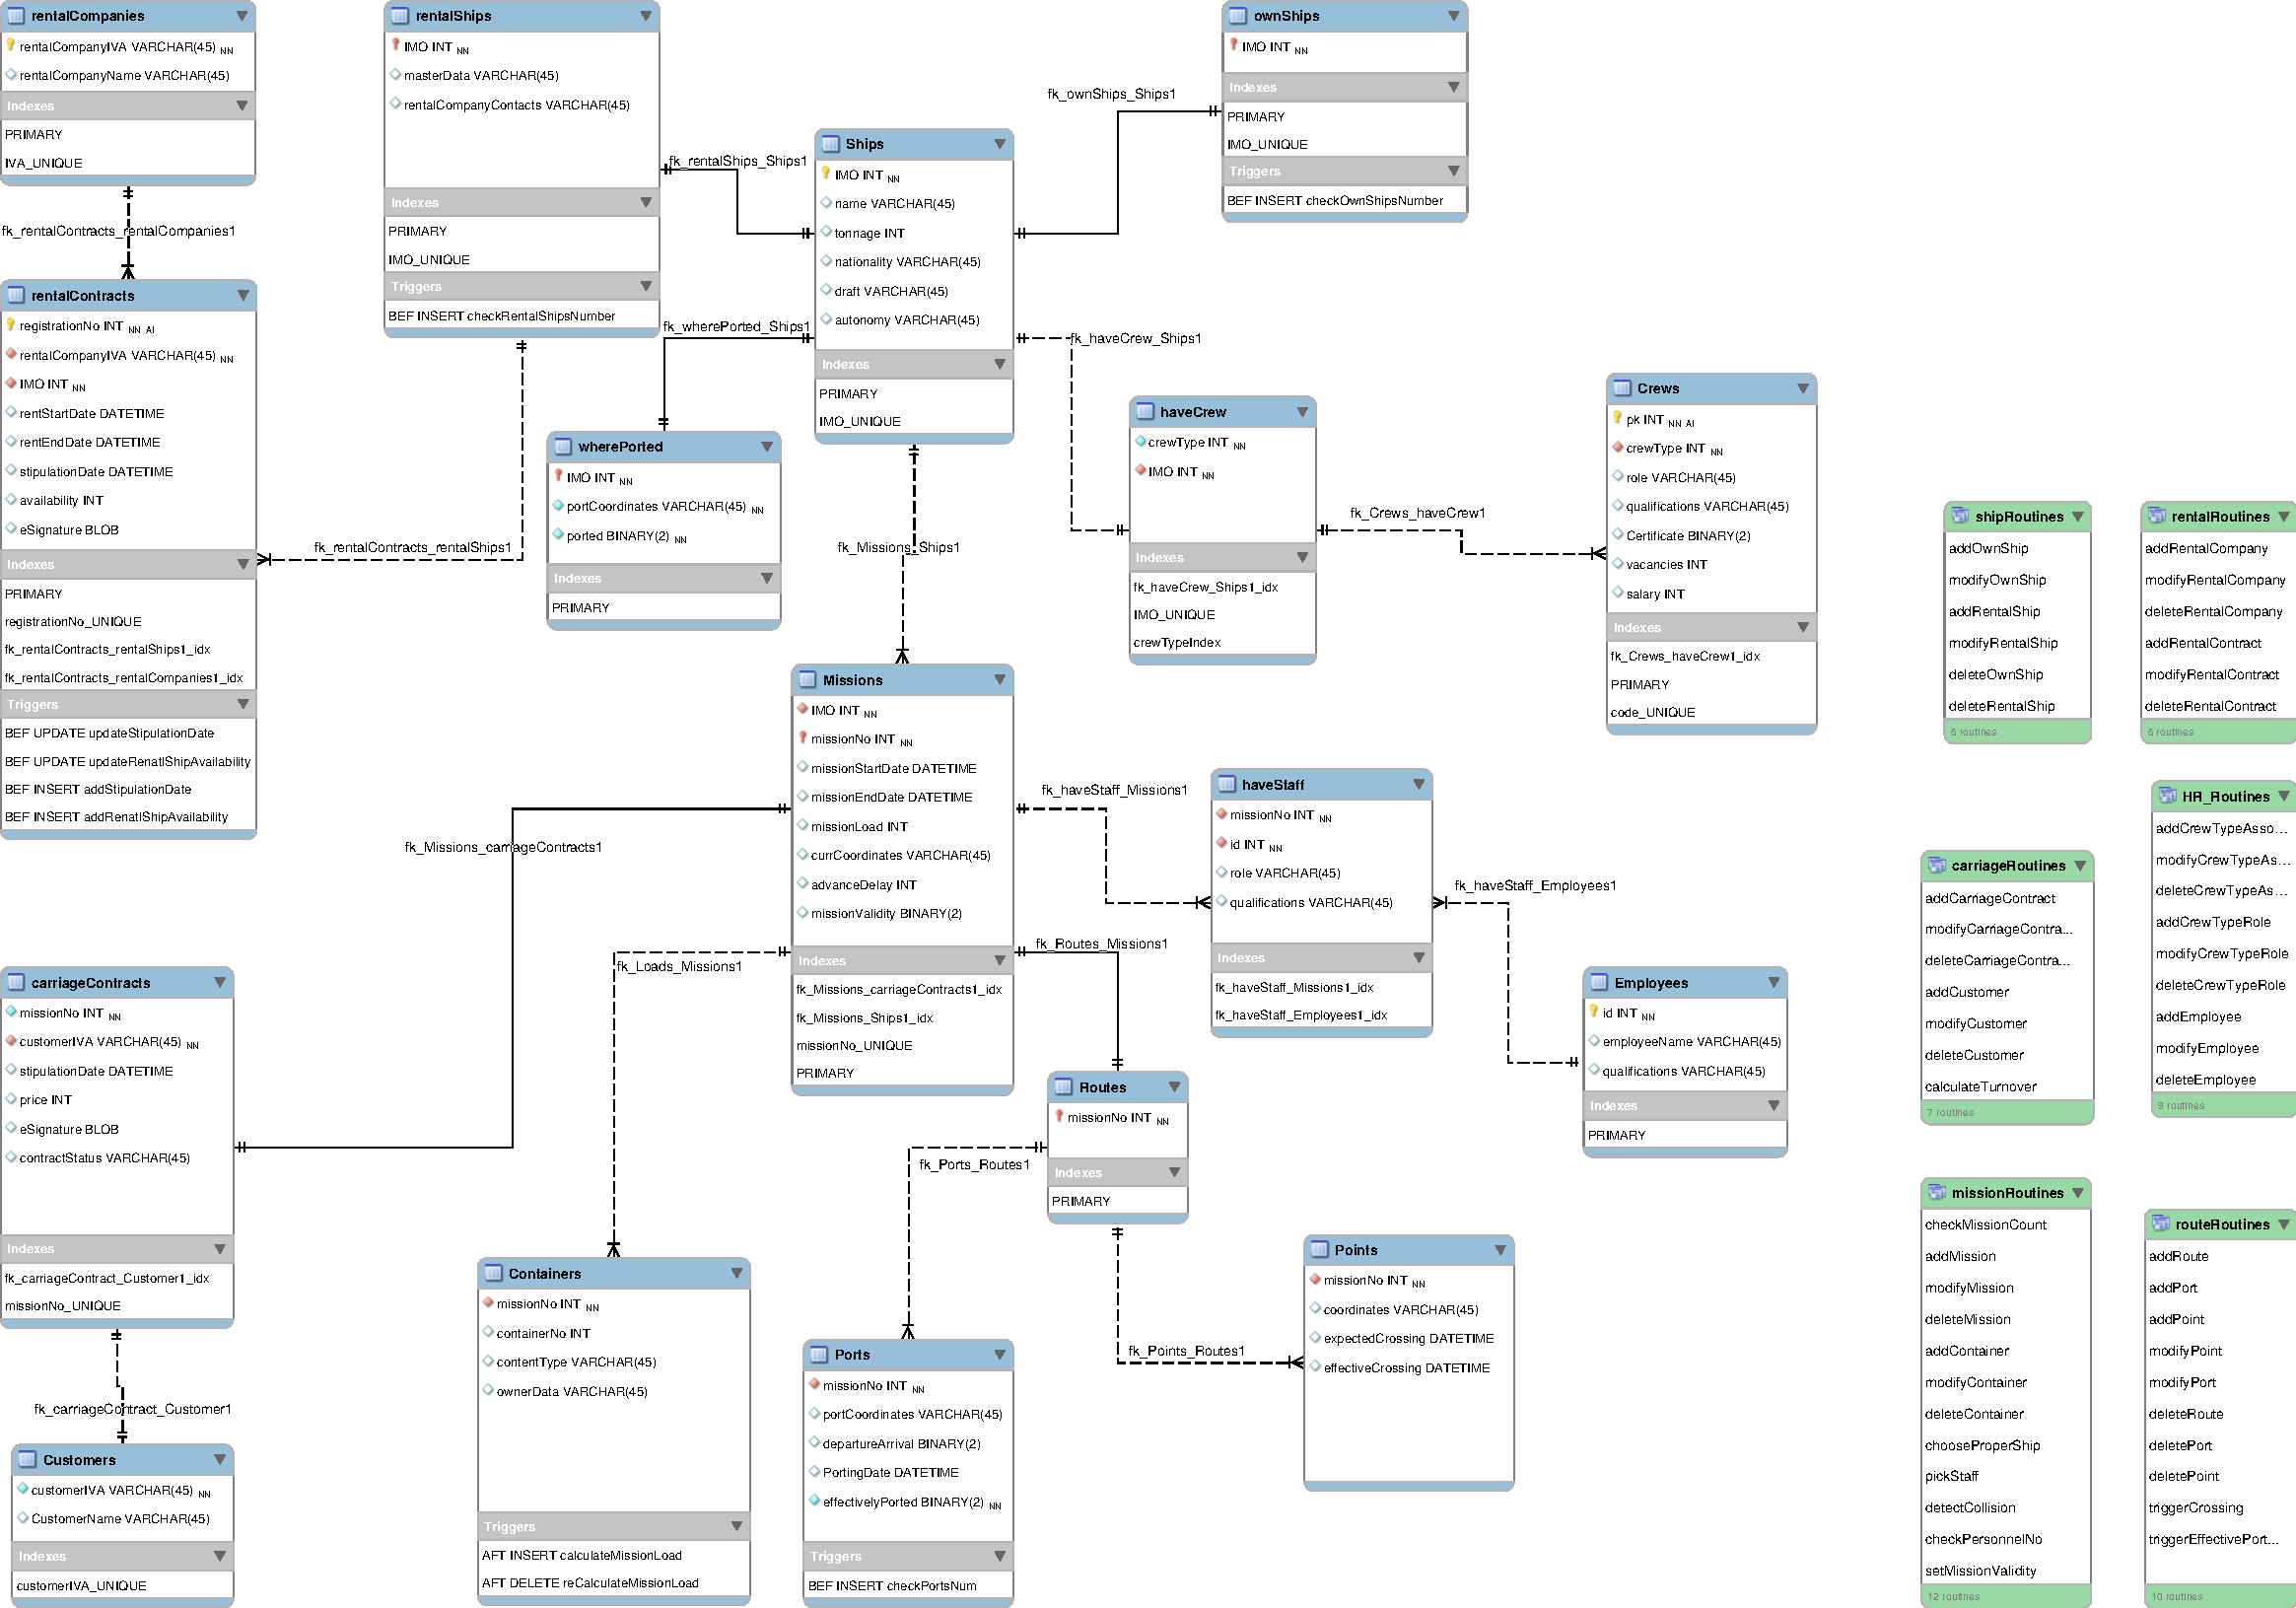
\includegraphics[height=\textheight, width=\textwidth]{MercantileShips-EER.pdf}
	\end{center}
\end{inlinefigure}
\newpage
\begin{inlinefigure}{Logical EERD with Column Matching Notation }
	\begin{center}
		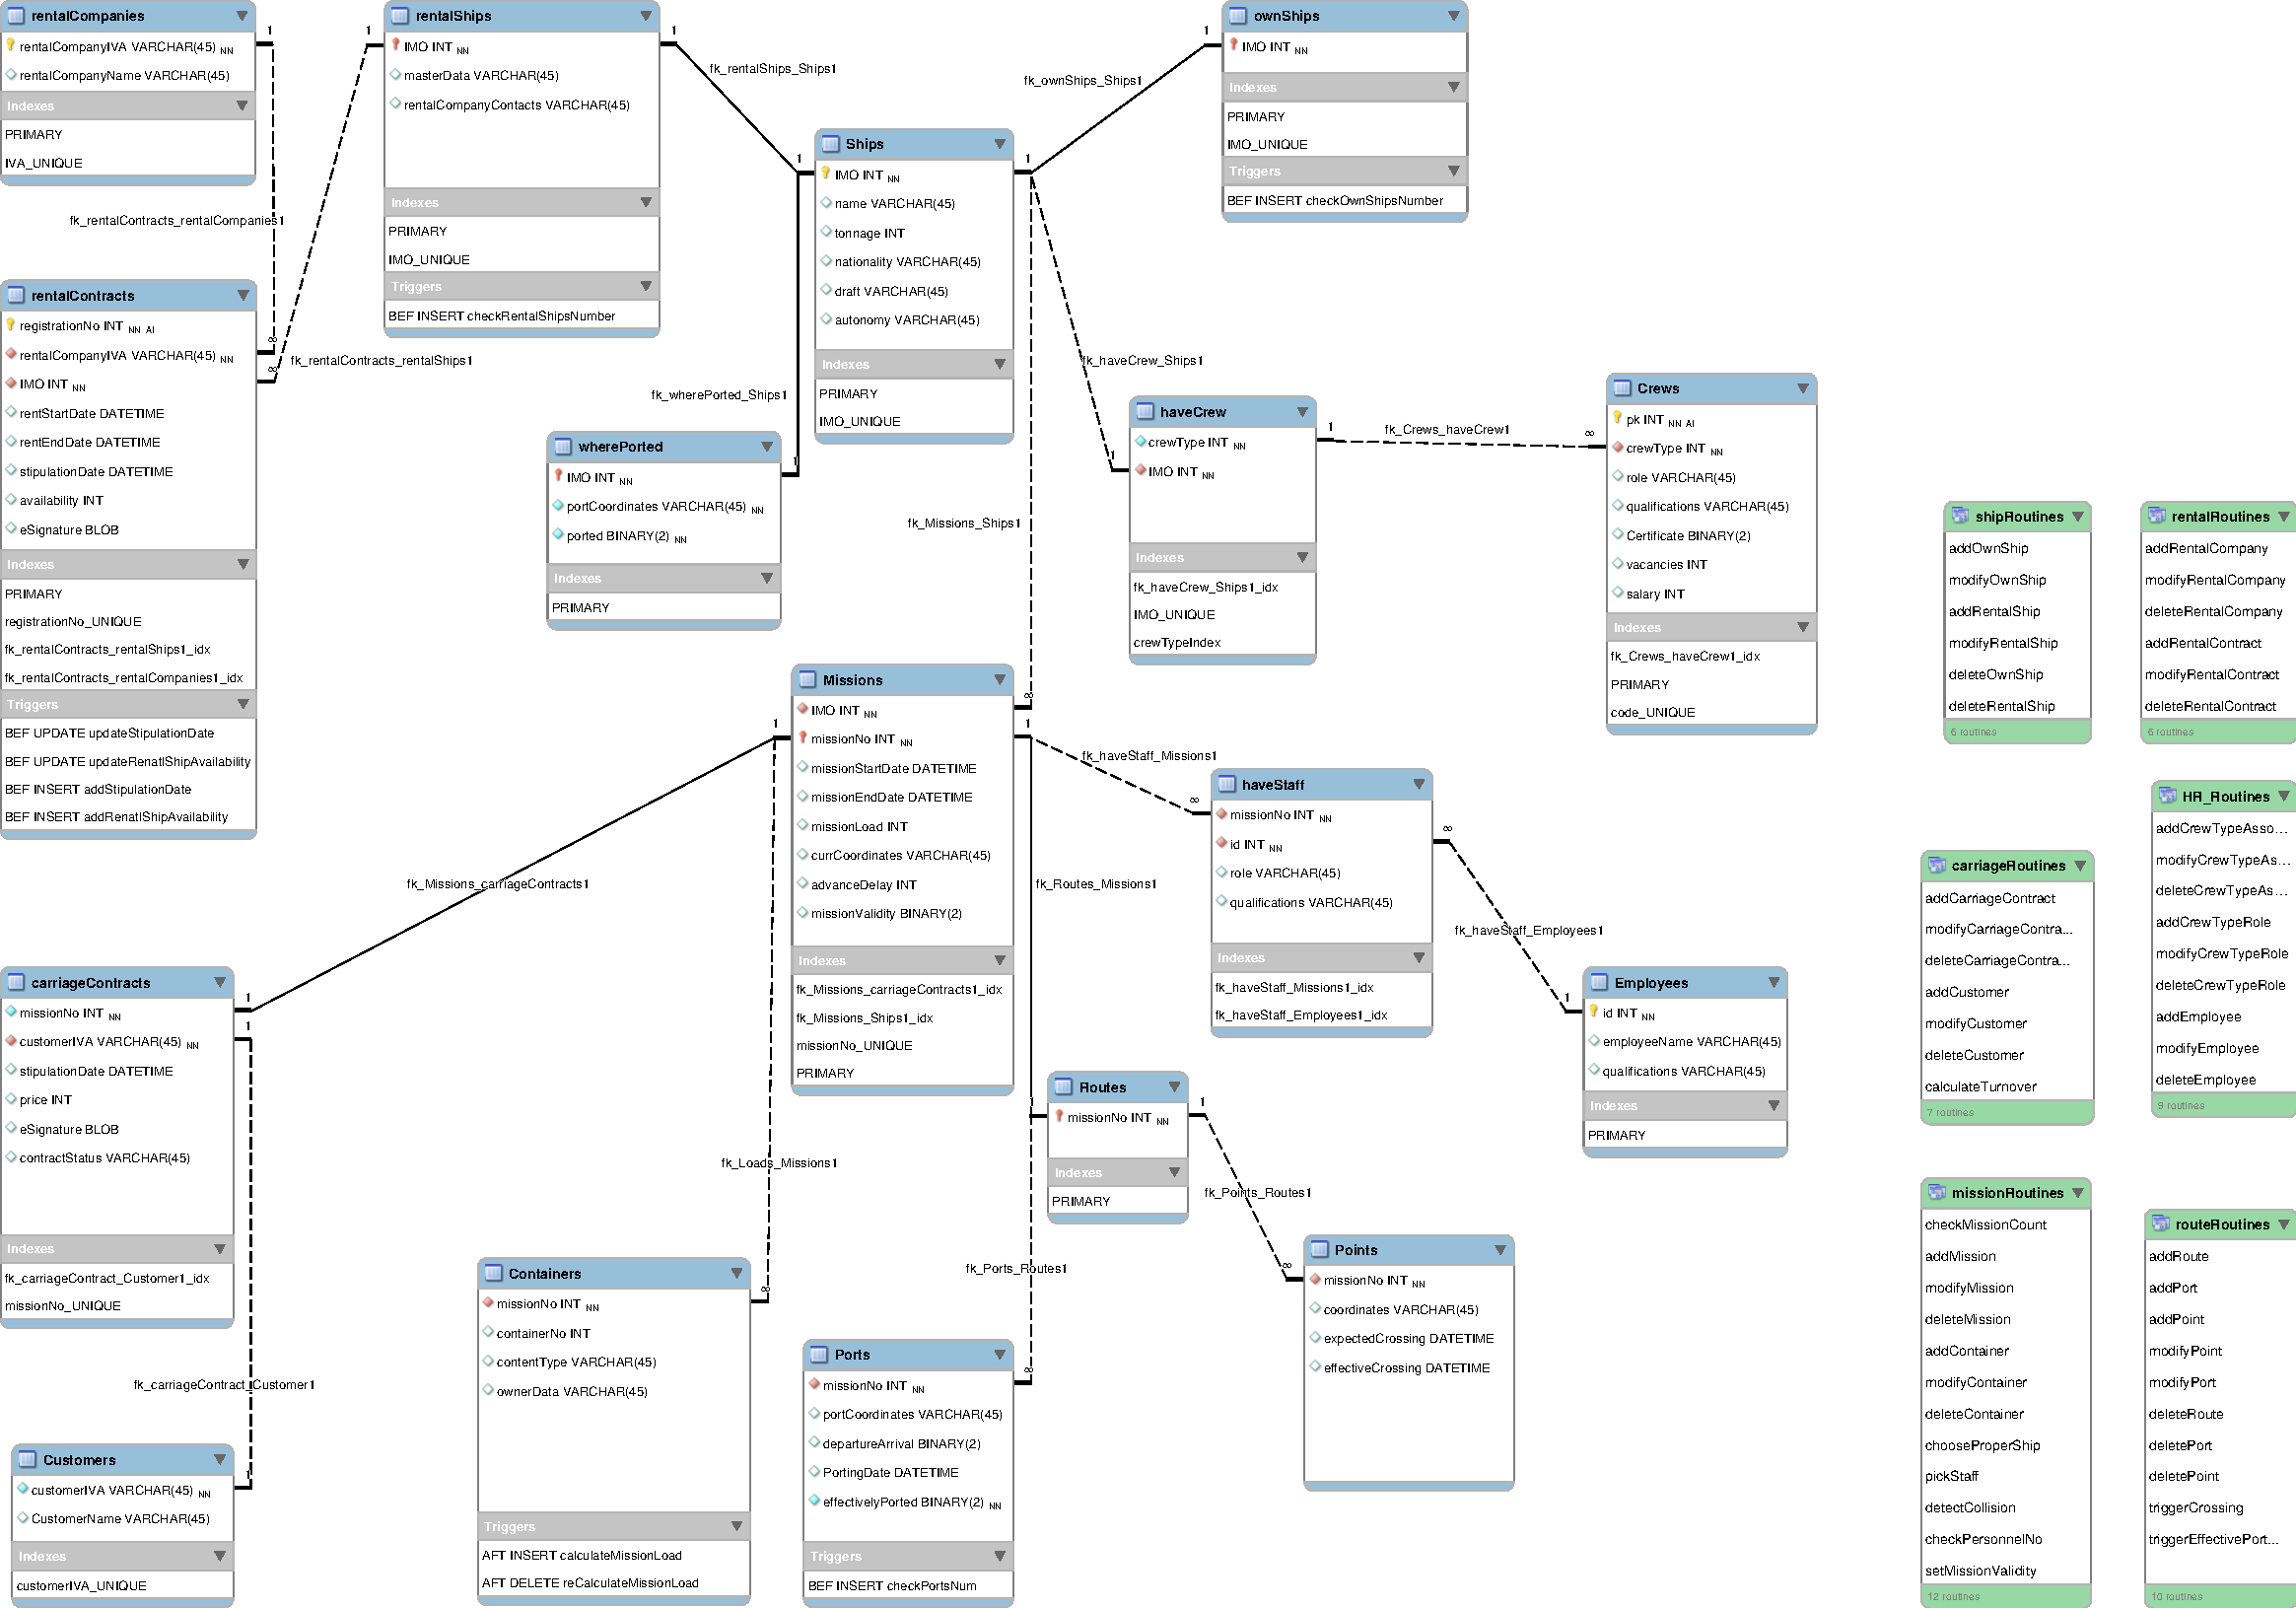
\includegraphics[height=\textheight, width=\textwidth]{MercantileShips-EER-Column.pdf}
	\end{center}
\end{inlinefigure}


\newpage
\chapter*{Stage 4: Physical Schema}
\inputminted[breaklines=true, fontsize=\footnotesize]{mysql}{../src/NavibusMercatoriis.sql}
\newpage
\begin{thebibliography}{}
	\bibitem {MySQL 5.7 Reference Manual}
		\textbf{MySQL 5.7 Reference Manual}: https://downloads.mysql.com/docs/refman-5.7-en.a4.pdf
	\bibitem {MySQL Workbench 6.3 Reference Manual}
		\textbf{MySQL Workbench 6.3 Reference Manual:} https://downloads.mysql.com/docs/workbench-en.a4.pdf
\end{thebibliography}
\end{document}
